% !TeX program = xelatex
% 中文阅读版：保留英文标题与小节标题；正文、图表注释及表内文字译为中文。
% 请使用 XeLaTeX 编译（中文正文及中文图文件名均不兼容 pdfLaTeX）。
\documentclass{article}
\usepackage[UTF8]{ctex}
\usepackage{spconf,amsmath,amssymb,graphicx,booktabs,multirow}
\usepackage{placeins,float}
\usepackage{cite}
\usepackage{url}
\newcommand{\metrictriplet}[3]{\makebox[3.1em][c]{#1}\hspace{0.5em}\makebox[3.1em][c]{#2}\hspace{0.5em}\makebox[3.1em][c]{#3}}
\newcommand{\metricheader}{\makebox[3.1em][c]{AP}\hspace{0.5em}\makebox[3.1em][c]{AP$_{50}$}\hspace{0.5em}\makebox[3.1em][c]{AP$_{75}$}}
\newcommand{\citerange}[2]{\mbox{\cite{#1}\textendash\kern-0.38em\cite{#2}}}

\title{PROMPTMINER-SAM2: PROMPT MINING FOR REMOTE SENSING INSTANCE SEGMENTATION}
\name{Anonymous Author(s)}
\address{Anonymous Affiliation(s)}

\begin{document}
\maketitle

\begin{abstract}
现有遥感实例分割方法通常从隐式实例表征直接预测掩码，虽能编码实例语义，但缺少局部形状的显式约束，因而易在复杂背景或相邻实例中混淆边界。
为此，本文提出面向遥感实例分割的 SAM2 自动提示框架 PromptMiner-SAM2，将候选区域的局部形状显式转化为掩码解码条件。
具体而言，粗形状提示挖掘模块从候选区域级特征预测局部粗形状，并据此生成形状感知提示；在此基础上，不确定性引导的解码器尾部细化模块仅修正初始掩码中置信度较低的位置。
在 WHU 和 NWPU VHR-10 上，PromptMiner-SAM2 的掩码 AP 分别为 73.4\% 和 68.3\%，在所比较方法中均为最高。
\end{abstract}
\begin{keywords}
实例分割，遥感影像，SAM2，提示挖掘，掩码细化
\end{keywords}

\section{INTRODUCTION}

遥感实例分割需要为场景中的每个目标预测像素级实例掩码，服务于城市规划和灾害评估等应用~\cite{rsiisn},~\cite{p2pformer}。
高分辨率遥感影像往往同时具有显著的尺度变化和复杂的背景纹理。
这些因素使目标与背景、相邻实例之间的局部边界难以区分，进而增加了实例掩码的精确预测难度。

现有实例分割方法可按掩码生成机制分为两阶段、单阶段、条件掩码预测和集合预测等范式。它们通常利用候选区域特征、动态参数或实例查询表征目标，并据此预测实例掩码~\citerange{maskrcnn}{condinst},~\cite{mask2former}。
面向遥感影像，已有工作从多尺度特征融合、边界建模和基础模型适配等方向改进实例掩码预测~\cite{rsiisn},~\cite{p2pformer},~\cite{rs4d},~\cite{directsamrs}。自动提示学习以及检测器与 SAM 之间的提示衔接，则拓展了提示式遥感实例分割的实现路径~\citerange{sam}{pasam},~\cite{rsprompter},~\cite{airwaysam}。

尽管实现范式不同，现有方法大多从隐式实例表征直接预测掩码。局部形状信息因而仍混合在语义表征中，难以作为可独立控制的空间条件直接参与掩码解码。
显式空间提示已被用于掩码细化；例如，SAMRefiner 从初始掩码中派生多类提示，以细化已有预测~\cite{samrefiner}。
本文关注一个与掩码细化互补的问题：如何从候选区域级特征中显式学习局部粗形状，并以此挖掘形状感知提示，为提示式实例掩码预测提供独立的空间条件？

\begin{figure}[t]
\centering
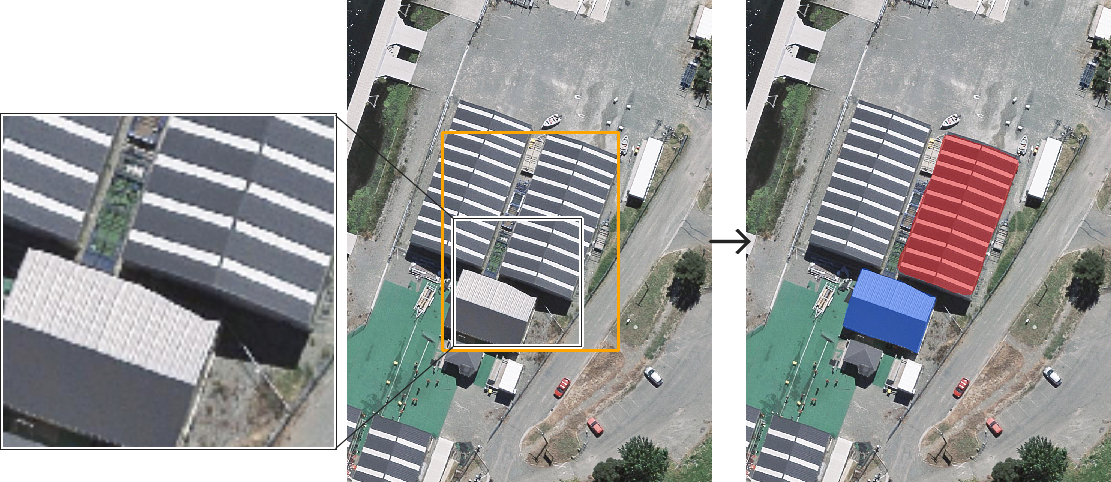
\includegraphics[width=\columnwidth]{teaser_300838_minimal_zoom.png}\par
\vspace{-0.15em}
{\small
\makebox[.5\columnwidth][c]{(a)}%
\makebox[.5\columnwidth][c]{(b)}\par}
\vspace{-0.3em}
\caption{实例局部形状的动机示例。(a) 候选框给出相邻建筑的空间范围，但未显式提供用于掩码解码的局部形状条件（局部放大）。(b) 真实实例掩码呈现了区分相邻实例所需的局部形状和边界信息。}
\label{fig:motivation}
\end{figure}

为此，PromptMiner-SAM2 从候选区域级特征中学习局部粗形状，并将其作为连接实例表征与提示式掩码解码的中间表示。模型随后基于该形状挖掘形状感知提示，为掩码解码提供独立的空间条件。
图~\ref{fig:arch} 给出了整体框架。

\begin{figure*}[!t]
\centering
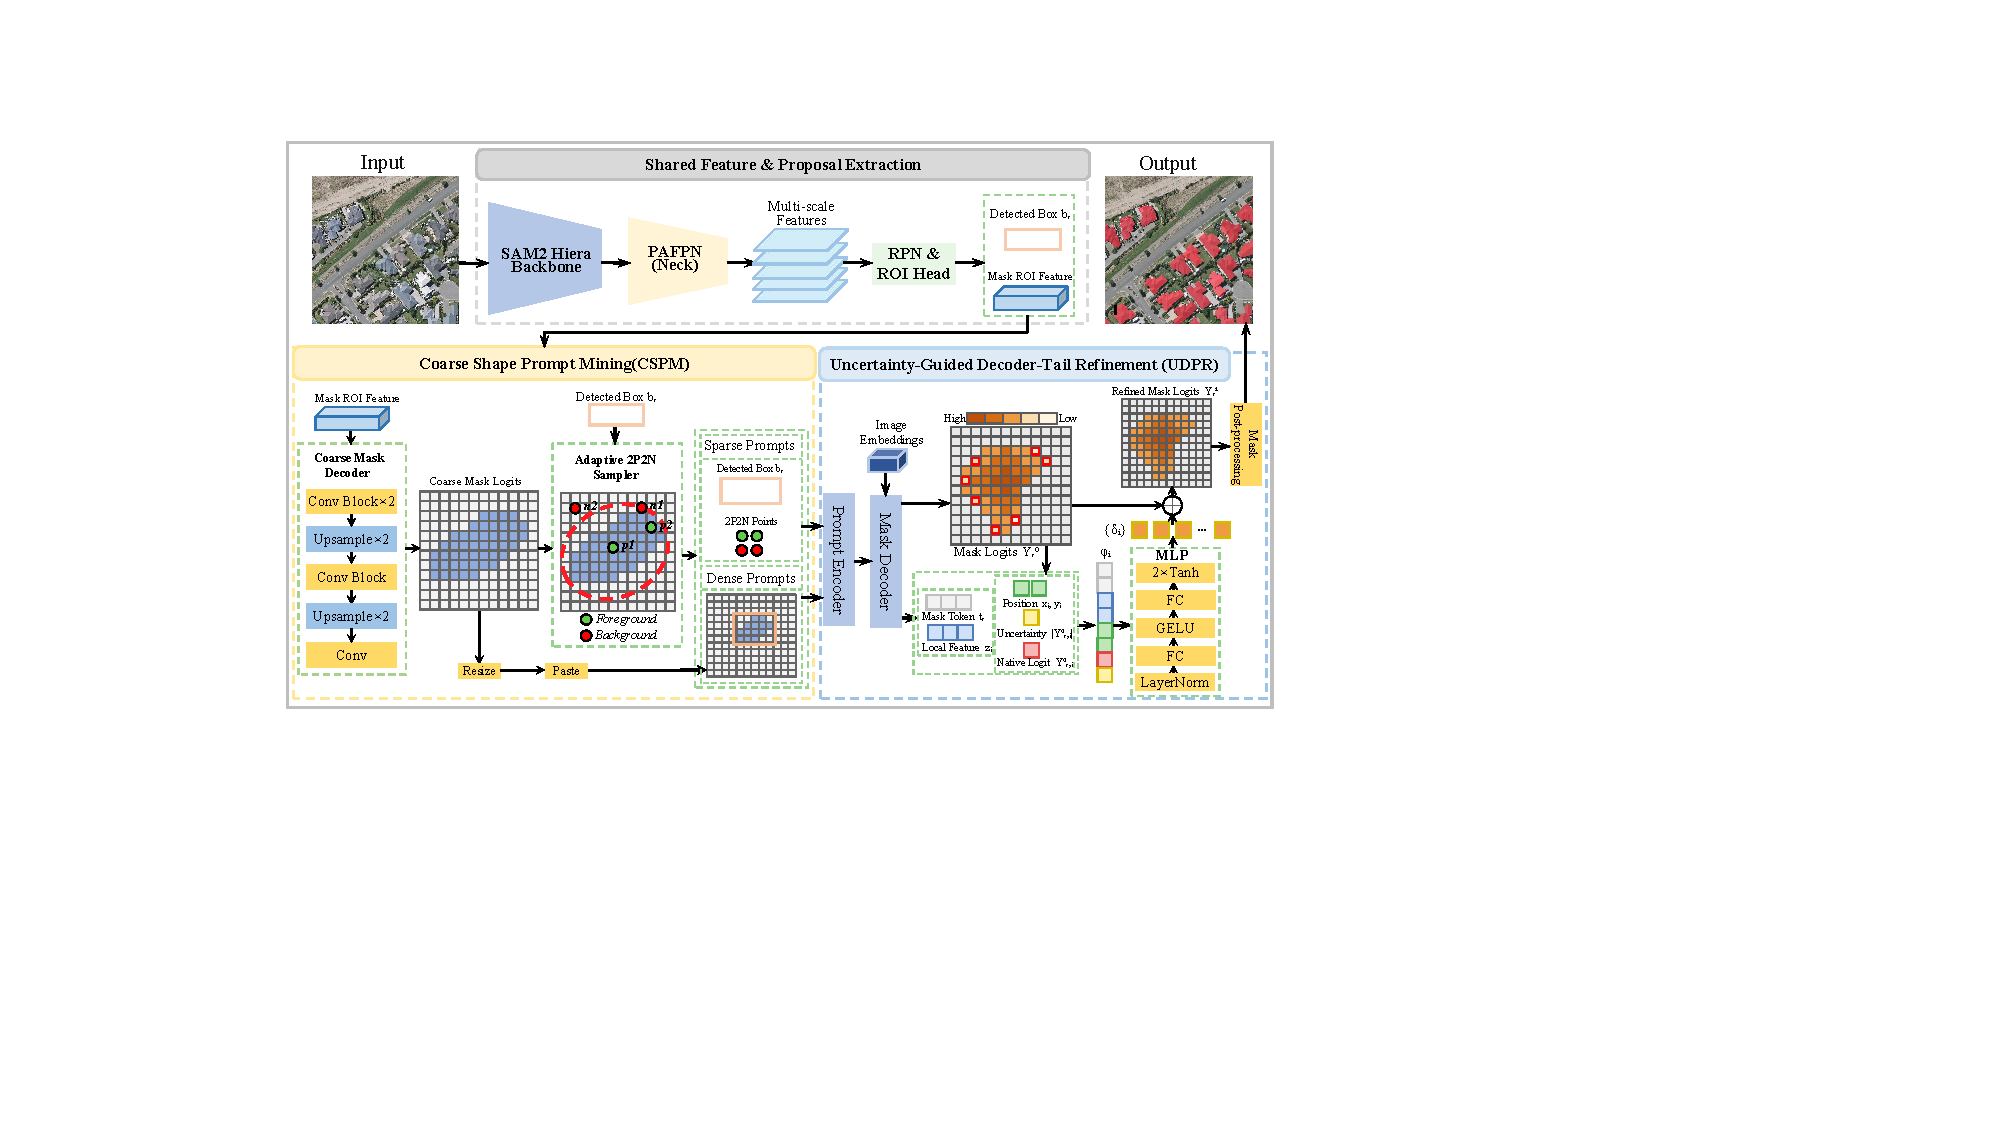
\includegraphics[width=\textwidth]{总体架构图.pdf}
\caption{PromptMiner-SAM2 的整体框架。图中展示了从输入影像、候选区域级特征和 SAM2 掩码解码到最终实例掩码的主要数据流。CSPM 负责挖掘局部形状条件并生成自动提示，UDR 负责对初始掩码中的不确定区域进行选择性修正。}
\label{fig:arch}
\end{figure*}

本文贡献如下：
\begin{itemize}
  \item 我们提出 PromptMiner-SAM2，一个面向遥感实例分割的 SAM2 自动提示框架。该框架将两阶段检测器与 SAM2 提示式掩码解码器结合，以候选区域级特征为条件自动构建解码提示并预测实例掩码。
  \item 我们设计 CSPM 和 UDR。CSPM 从候选区域级特征中学习候选区域局部粗形状，并据此挖掘形状感知提示；UDR 对初始掩码中的不确定位置进行选择性修正，以提升掩码质量。
  \item 我们在 WHU 和 NWPU VHR-10 两个遥感基准上验证了 PromptMiner-SAM2 的性能，并系统分析不同提示组合与 UDR 对实例定位和掩码预测的影响。结果表明，完整框架在所比较方法中取得最高掩码 AP；消融实验进一步量化了稀疏提示、稠密形状条件与局部不确定性修正的互补作用。
\end{itemize}

\section{METHOD}

\subsection{Overall Architecture}
如图~\ref{fig:arch} 所示，PromptMiner-SAM2 将两阶段检测器与 SAM2 的提示式掩码解码器结合，形成从实例定位到掩码预测的统一流程。
对于输入影像，SAM2 的 Hiera 图像编码器首先提取多尺度特征。检测分支经 PAFPN、RPN 和 RoI 路径生成候选区域级特征及其空间范围；Hiera 特征同时为 SAM2 掩码解码提供图像嵌入。
CSPM 基于候选区域级特征挖掘自动提示。SAM2 将这些提示与图像嵌入共同解码为初始实例掩码，UDR 再对其中的不确定局部区域进行选择性修正，得到最终掩码。


\subsection{Coarse-Shape Prompt Mining}
CSPM 从候选区域级特征中学习局部粗形状，并从中挖掘用于 SAM2 掩码解码的形状感知提示。下文以 $r$ 表示一个候选区域，其 RoI 特征记为 $X_r$，对应的检测框记为 $b_r$。其中，$X_r$ 编码候选区域内的局部视觉与形状信息，$b_r$ 定义该区域的空间范围和坐标参照。挖掘得到的提示包括稀疏点提示和稠密形状提示。

\indent 首先，粗形状分支将 RoI 特征 $X_r$ 映射为在候选框局部坐标系中定义的形状 logit 图：
\begin{equation}
C_r=f_{\mathrm{coarse}}(X_r),\qquad C_r\in\mathbb{R}^{1\times64\times64}.
\label{eq:coarse}
\end{equation}
\indent 训练时，将对应实例的真实掩码按候选框裁剪并映射至相同的局部坐标系，以监督粗形状分支。该分支的独立损失引导 $C_r$ 学习候选区域内的前景布局和边界结构。

\indent 随后，以 $p_r=\sigma(C_r)$ 将粗形状 logits 转换为前景概率，并以概率阈值 $0.5$ 确定前景支持区域。对于局部形状图上的像素位置 $u$，$\bar d_r(u)$ 表示其到预测前景边界的内部距离，并以局部形状图的短边长度归一化。两个正点依次从满足前景置信度和内部距离约束的像素中，按 $p_r(u)\bar d_r(u)$ 评分选取；第二个正点额外避开首个正点的预设邻域。两个负点依次从一像素宽的低概率外环和膨胀前景之外的低概率背景中，按 $1-p_r(u)$ 评分选取；第二个负点还避开首个正点和首个负点。

\indent 随后，$b_r$ 作为三类提示的共同空间参照。选中的局部点映射至图像坐标，并连同正负标签构成稀疏提示集合 $\mathcal{S}_r$；局部粗形状 logits 经缩放后放置在 $b_r$ 覆盖的图像区域，形成稠密提示 $Q_r$；$b_r$ 本身则作为框提示输入。SAM2 将三类提示与图像嵌入共同解码：
\begin{equation}
Y_r^0=\mathcal{D}\bigl(\mathcal{E}_I(I),
\widetilde{\mathcal{E}}_P(\mathcal{S}_r,b_r,Q_r)\bigr),
\label{eq:native-decoding}
\end{equation}
\indent 其中，$\mathcal{E}_I$、$\widetilde{\mathcal{E}}_P$ 和 $\mathcal{D}$ 分别表示图像编码器、提示嵌入路径和掩码解码器；由有符号粗形状 logits 形成的 $Q_r$ 保留连续的前景/背景置信度信息。

\subsection{Uncertainty-Guided Decoder-Tail Refinement}
UDR 用于修正 SAM2 初始实例掩码预测中置信度最低的局部位置。一次提示式解码同时产生初始 logit 图 $Y_r^0$、与其空间对齐的解码器特征图 $U_r$ 和实例相关的掩码 token $t_r$。UDR 基于这些解码输出，仅在选定位置预测局部残差，其余位置保持原始解码结果不变。

\indent 首先，UDR 在初始 logit 图 $Y_r^0$ 的解码器输出网格 $\mathcal{G}_r$ 上定位不确定区域。logit 绝对值较小的位置更接近前景/背景决策边界，因此选取其中最不确定的 $K_r$ 个位置：
\begin{equation}
\begin{aligned}
K_r&=\min(K,|\mathcal{G}_r|),\\
\Omega_r&=\operatorname{BottomK}\bigl(|Y_r^0|,K_r\bigr),\qquad K=64,
\end{aligned}
\label{eq:udpr-selection}
\end{equation}
\indent 其中，$\operatorname{BottomK}$ 返回 $\mathcal{G}_r$ 中 logit 绝对值最小的 $K_r$ 个位置索引。

\indent 对每个选定位置 $i\in\Omega_r$，从对齐特征图 $U_r$ 中提取局部特征 $z_i$，并将其与实例 token、归一化坐标、对应 logit 及其绝对值拼接：
\begin{equation}
\phi_i=[z_i,t_r,Y^0_{r,i},x_i,y_i,|Y^0_{r,i}|].
\label{eq:udpr-input}
\end{equation}
\indent 其中，$x_i$ 和 $y_i$ 分别表示位置 $i$ 在 $\mathcal{G}_r$ 中归一化后的横、纵坐标。该特征同时包含局部解码证据、实例级上下文和当前预测状态，使残差预测能够针对具体实例和位置进行调整。随后，轻量级 MLP $g$ 为每个选定位置预测有界残差；掩码监督引导残差将预测修正为正确的前景或背景状态：
\begin{equation}
\delta_i=2\tanh g(\phi_i),\qquad i\in\Omega_r,
\label{eq:udpr}
\end{equation}

\indent 最后，将预测残差写回对应位置，形成细化后的 logit 图：
\begin{equation}
Y^1_{r,i}=\begin{cases}
Y^0_{r,i}+\delta_i, & i\in\Omega_r,\\
Y^0_{r,i}, & i\notin\Omega_r.
\end{cases}
\label{eq:udpr-scatter}
\end{equation}
\indent 该选择性更新仅修正 $\Omega_r$ 中的位置，并保持其余解码器输出不变，从而在现有 SAM2 解码器输出网格上完成有界的局部残差修正。

\section{EXPERIMENTS}
\subsection{Experimental Setup}
我们在 WHU 和 NWPU VHR-10 两个遥感基准上评估方法。WHU 是单类别建筑实例分割基准，包含 2,943/627/2,220 张训练、验证和测试图像~\cite{whu}。NWPU VHR-10 是十类别目标检测基准~\cite{nwpu}，原始版本仅提供检测标注；因此，本文采用 Su \textit{et al.}~\cite{nwpu_instance} 公开发布的实例掩码及其 520/130 训练/评估划分。

我们采用 PyTorch 实现模型，并在四张 NVIDIA RTX 3090 GPU 上以分布式数据并行训练。每张 GPU 处理一张图像，结合两步梯度累积后，有效批量大小为八。两个基准均由 SAM2 Hiera-Base+ 权重初始化：Hiera 主干参数保持冻结，其适配模块、提示路径和掩码解码器参与训练。优化器采用初始学习率为 $5\times10^{-4}$ 的 AdamW，并使用余弦退火学习率策略；训练目标联合包含检测、粗形状提示和最终实例掩码损失。

在统一开发协议下，我们从 $K\in\{32,64,128\}$ 中选择 UDR 的修正位置数。表~\ref{tab:k-sensitivity} 显示，$K=64$ 取得最高的总体 bbox AP 和掩码 AP，因此用于主要实验。

\begin{table}[H]
\caption{在统一开发协议下，$K$ 在 NWPU VHR-10 数据集上的敏感性分析。}
\label{tab:k-sensitivity}
\centering
\small
\begin{tabular}{c ccc ccc}
\toprule
& \multicolumn{3}{c}{边界框（\%）} & \multicolumn{3}{c}{掩码（\%）} \\
\cmidrule(lr){2-4}\cmidrule(lr){5-7}
$K$ & AP & AP$_{50}$ & AP$_{75}$ & AP & AP$_{50}$ & AP$_{75}$ \\
\midrule
32  & 69.38 & 91.69 & 79.03 & 64.94 & 92.91 & 70.01 \\
64  & \textbf{70.35} & 92.23 & \textbf{81.65} & \textbf{66.65} & \textbf{94.15} & 71.97 \\
128 & 70.13 & \textbf{92.42} & 81.32 & 65.97 & 93.71 & \textbf{72.22} \\
\bottomrule
\end{tabular}
\end{table}

\subsection{Comparative Analysis}
我们将 PromptMiner-SAM2 与 10 种代表性实例分割方法进行比较。为便于分析，将对比方法归为基于 CNN 的方案（CNN）和基于全局序列建模的方案（GSM）。前者包括两阶段、单阶段和级联设计，后者包括 Transformer 风格的掩码预测和基础模型提示。表~\ref{tab:comparison} 的\emph{类别}列采用这两个缩写。

\begin{figure*}[t]
\centering
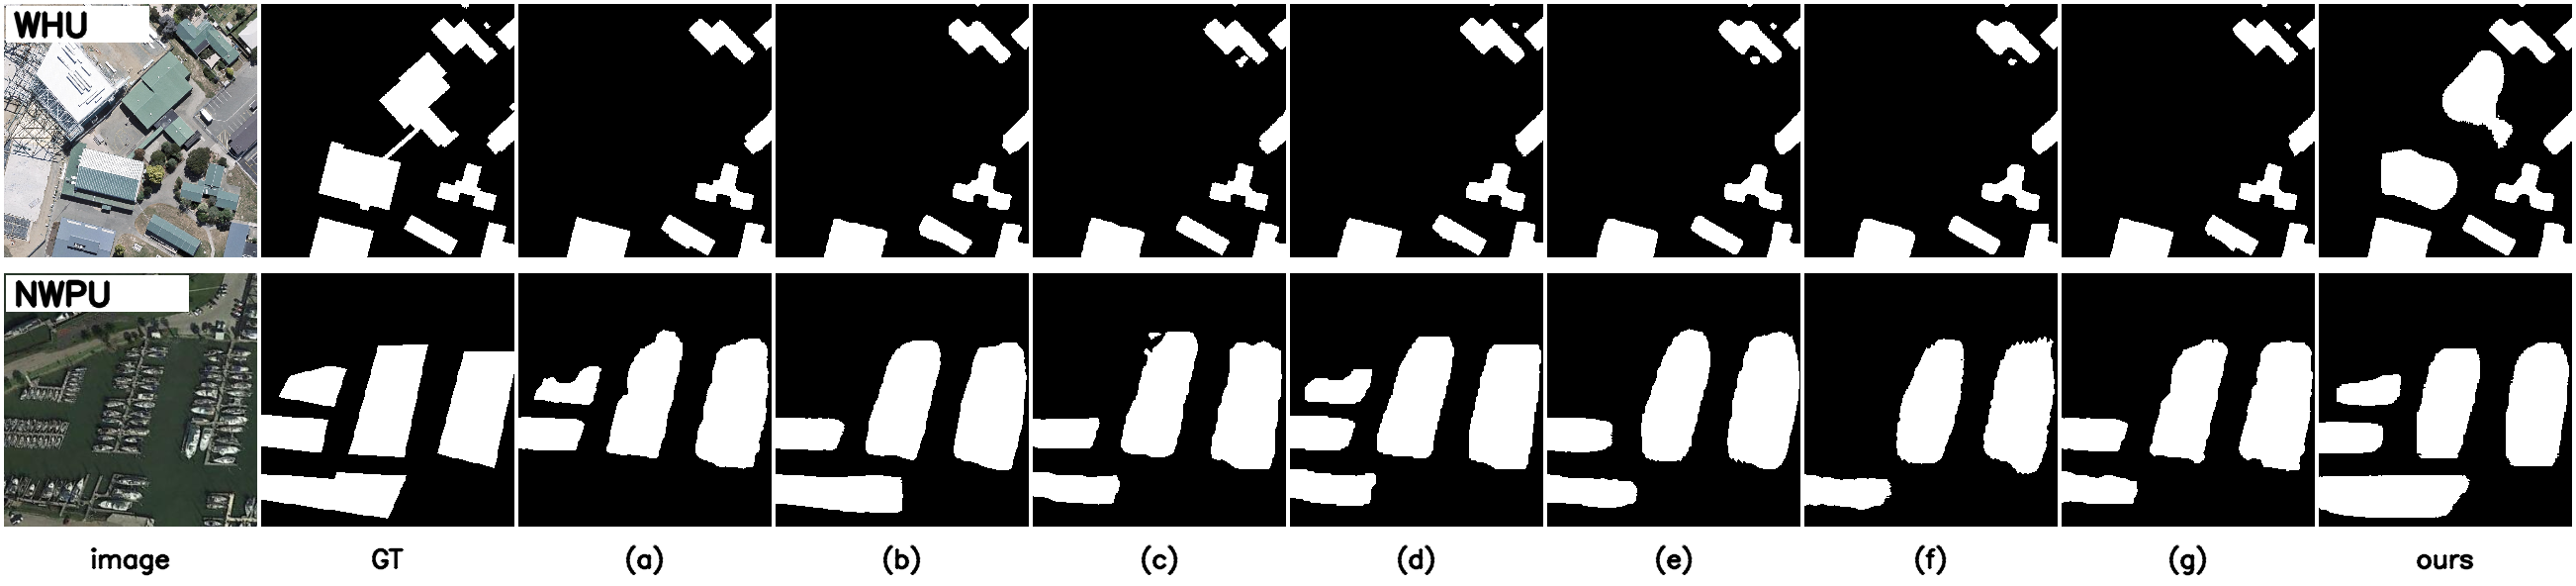
\includegraphics[width=\textwidth]{viz_grid_row_combined.png}\par
\vspace{-0.15em}
{\small
\makebox[.1\textwidth][c]{输入}%
\makebox[.1\textwidth][c]{真实标注}%
\makebox[.1\textwidth][c]{(a)}%
\makebox[.1\textwidth][c]{(b)}%
\makebox[.1\textwidth][c]{(c)}%
\makebox[.1\textwidth][c]{(d)}%
\makebox[.1\textwidth][c]{(e)}%
\makebox[.1\textwidth][c]{(f)}%
\makebox[.1\textwidth][c]{(g)}%
\makebox[.1\textwidth][c]{本文方法}\par}
\vspace{-0.3em}
\caption{WHU 和 NWPU VHR-10 数据集上的定性比较。从左至右，各列依次为输入图像、真实标注、(a) MaskDINO、(b) RSPrompter、(c) CondInst、(d) YOLO11、(e) HTC、(f) Mask R-CNN、(g) M2F 以及 PromptMiner-SAM2（本文方法）的预测结果。}
\label{fig:qualitative}
\end{figure*}

\begin{table*}[t]
\caption{WHU 数据集和 NWPU VHR-10 数据集上的比较分析。边界框和掩码列的每个条目均报告 AP / AP$_{50}$ / AP$_{75}$（\%）。}
\label{tab:comparison}
\centering
\small
\begingroup
\setlength{\tabcolsep}{3pt}
\renewcommand{\arraystretch}{1.08}
\begin{tabular}{llcccc}
\toprule
& & \multicolumn{2}{c}{WHU} & \multicolumn{2}{c}{NWPU VHR-10} \\
\cmidrule(lr){3-4}\cmidrule(lr){5-6}
& & 边界框（\%） & 掩码（\%） & 边界框（\%） & 掩码（\%） \\
\cmidrule(lr){3-3}\cmidrule(lr){4-4}\cmidrule(lr){5-5}\cmidrule(lr){6-6}
类别 & 方法 & \metricheader & \metricheader & \metricheader & \metricheader \\
\midrule
\multirow{5}{*}{\textit{CNN}} & Mask R-CNN~\cite{maskrcnn} & \metrictriplet{70.9}{89.9}{80.9} & \metrictriplet{68.2}{90.0}{80.0} & \metrictriplet{65.4}{90.2}{78.9} & \metrictriplet{63.0}{90.1}{71.2} \\
& MS R-CNN~\cite{msrcnn} & \metrictriplet{68.8}{89.4}{80.0} & \metrictriplet{67.7}{89.6}{79.5} & \metrictriplet{67.8}{94.3}{83.8} & \metrictriplet{64.7}{93.6}{\textbf{80.8}} \\
& HTC~\cite{htc} & \metrictriplet{72.7}{90.6}{82.5} & \metrictriplet{69.2}{90.7}{81.6} & \metrictriplet{58.9}{86.9}{67.7} & \metrictriplet{51.3}{84.6}{53.3} \\
& CondInst~\cite{condinst} & \metrictriplet{74.2}{90.0}{82.4} & \metrictriplet{69.7}{90.2}{80.9} & \metrictriplet{65.0}{90.1}{79.6} & \metrictriplet{62.8}{90.7}{68.1} \\
& YOLO11s-seg~\cite{yolo11} & \metrictriplet{\textbf{76.7}}{91.2}{\textbf{85.4}} & \metrictriplet{66.8}{91.3}{79.1} & \metrictriplet{71.0}{\textbf{94.4}}{79.5} & \metrictriplet{63.9}{93.9}{67.3} \\
\midrule
\multirow{5}{*}{\textit{GSM}} & Mask2Former~\cite{mask2former} & \metrictriplet{61.4}{82.7}{70.7} & \metrictriplet{64.5}{84.1}{75.6} & \metrictriplet{60.3}{77.9}{66.8} & \metrictriplet{61.5}{84.9}{67.8} \\
& MaskDINO~\cite{maskdino} & \metrictriplet{73.3}{90.8}{82.7} & \metrictriplet{73.3}{90.3}{82.5} & \metrictriplet{65.7}{88.9}{74.2} & \metrictriplet{65.8}{89.6}{71.5} \\
& RS4D-box~\cite{rs4d} & \metrictriplet{64.5}{87.6}{74.7} & \metrictriplet{64.1}{87.8}{75.2} & \metrictriplet{57.0}{82.5}{65.4} & \metrictriplet{54.3}{80.1}{57.6} \\
& RSIISN~\cite{rsiisn} & \metrictriplet{74.1}{90.0}{84.4} & \metrictriplet{72.1}{90.1}{83.9} & \metrictriplet{66.7}{91.5}{78.4} & \metrictriplet{62.9}{89.7}{67.1} \\
& RSPrompter~\cite{rsprompter} & \metrictriplet{72.5}{91.0}{81.7} & \metrictriplet{72.5}{\textbf{92.0}}{82.9} & \metrictriplet{70.3}{93.6}{81.0} & \metrictriplet{66.1}{92.7}{70.6} \\
\midrule
本文 & PromptMiner-SAM2 & \metrictriplet{76.4}{\textbf{91.5}}{\textbf{85.4}} & \metrictriplet{\textbf{73.4}}{91.4}{\textbf{85.5}} & \metrictriplet{\textbf{73.4}}{94.0}{\textbf{84.2}} & \metrictriplet{\textbf{68.3}}{\textbf{94.5}}{74.6} \\
\bottomrule
\end{tabular}
\endgroup
\end{table*}

表~\ref{tab:comparison} 显示，PromptMiner-SAM2 在 WHU 和 NWPU VHR-10 上均取得最高掩码 AP，分别比最强对比方法高 0.1 和 2.2 个百分点。在 WHU 上，掩码 AP$_{75}$ 同样为最优；边界框 AP 为 76.4%，仅略低于 YOLO11s-seg 的 76.7%。在 NWPU VHR-10 上，本文方法在边界框 AP、边界框 AP$_{75}$、掩码 AP 和掩码 AP$_{50}$ 上均为最优。其掩码 AP$_{75}$ 并非全表最高，但高于所有 GSM 对比方法。

图~\ref{fig:qualitative} 展示了 WHU 和 NWPU VHR-10 上的定性比较。在 WHU 样例中，本文方法能够分离相接触的建筑屋顶；在 NWPU 样例中，目标区域预测更完整，并减少了相邻实例被合并的错误。

\begin{table}[H]
\caption{NWPU VHR-10 数据集上的提示路径消融；$P$、$B$ 和 $M$ 分别表示点、框和稠密掩码提示，UDR 表示不确定性引导的解码器尾部细化。}
\label{tab:ablation}
\centering
\small
\setlength{\tabcolsep}{3pt}
\begin{tabular}{lcccccc}
\toprule
& \multicolumn{3}{c}{边界框（\%）} & \multicolumn{3}{c}{掩码（\%）} \\
\cmidrule(lr){2-4}\cmidrule(lr){5-7}
变体 & AP & AP$_{50}$ & AP$_{75}$ & AP & AP$_{50}$ & AP$_{75}$ \\
\midrule
$P$ & 71.81 & 93.60 & 81.89 & 63.15 & 92.56 & 67.73 \\
$B$ & 72.14 & \textbf{94.34} & 82.24 & 65.25 & 94.12 & 69.02 \\
$P{+}B$ & 71.74 & 93.52 & 81.68 & 66.94 & 93.93 & 72.73 \\
$P{+}B{+}M$ & \textbf{73.76} & 93.80 & \textbf{84.69} & 66.35 & 93.66 & 71.61 \\
$P{+}B{+}M$ + UDR & 73.43 & 93.96 & 84.16 & \textbf{68.28} & \textbf{94.53} & \textbf{74.61} \\
\bottomrule
\end{tabular}
\end{table}

\subsection{Ablation Study}
\vspace{-0.35em}
表~\ref{tab:ablation} 总结了不同提示类型和解码器尾部细化的影响。相较于仅使用点提示 $P$，仅使用框提示 $B$ 时，掩码 AP 由 63.15\% 提升至 65.25\%，掩码 AP$_{75}$ 由 67.73\% 提升至 69.02\%。联合使用两类离散提示（$P{+}B$）后，掩码 AP 和掩码 AP$_{75}$ 分别达到 66.94\% 和 72.73\%，说明点提示与框提示能够提供互补的空间约束。

在 $P{+}B$ 的基础上加入稠密掩码提示 $M$ 后，边界框 AP 和边界框 AP$_{75}$ 分别达到 73.76\% 和 84.69\%，而掩码 AP 和掩码 AP$_{75}$ 分别为 66.35\% 和 71.61\%。进一步加入 UDR 后，完整的 $P{+}B{+}M{+}\mathrm{UDR}$ 配置取得 68.28\% 的掩码 AP 和 74.61\% 的掩码 AP$_{75}$，均为该消融实验中的最高值。

\section{CONCLUSION}
本文提出 PromptMiner-SAM2：该框架从候选区域级特征中学习局部粗形状，挖掘用于 SAM2 解码的形状感知提示，并对初始实例掩码中的不确定位置进行选择性修正。在 WHU 和 NWPU VHR-10 数据集上，方法分别取得 73.4\% 和 68.3\% 的掩码 AP。未来可进一步探索能够适应目标尺度和局部场景上下文的提示挖掘方式。

\clearpage
\bibliographystyle{IEEEbib}
\begin{thebibliography}{99}
\bibitem{rsiisn} W.~Ye, W.~Zhang, W.~Lei, W.~Zhang, X.~Chen, and Y.~Wang, ``Remote sensing image instance segmentation network with transformer and multi-scale feature representation,'' \textit{Expert Syst. Appl.}, vol.~234, Art.~no.~121007, 2023.
\bibitem{p2pformer} T.~Zhang, S.~Wei, Y.~Zhou, M.~Luo, W.~Yu, and S.~Ji, ``P2PFormer: A primitive-to-polygon method for regular building contour extraction from remote sensing images,'' \textit{IEEE Trans. Geosci. Remote Sens.}, vol.~62, Art.~no.~4414012, 2024.
\bibitem{maskrcnn} K.~He, G.~Gkioxari, P.~Doll\'ar, and R.~Girshick, ``Mask R-CNN,'' in \textit{Proc. IEEE Int. Conf. Comput. Vis. (ICCV)}, 2017, pp.~2961--2969.
\bibitem{msrcnn} Z.~Huang, L.~Huang, Y.~Gong, C.~Huang, and X.~Wang, ``Mask scoring R-CNN,'' in \textit{Proc. IEEE/CVF Conf. Comput. Vis. Pattern Recognit. (CVPR)}, 2019, pp.~6409--6418.
\bibitem{htc} K.~Chen \textit{et al.}, ``Hybrid task cascade for instance segmentation,'' in \textit{Proc. IEEE/CVF Conf. Comput. Vis. Pattern Recognit. (CVPR)}, 2019, pp.~4974--4983.
\bibitem{condinst} Z.~Tian, C.~Shen, and H.~Chen, ``Conditional convolutions for instance segmentation,'' in \textit{Proc. Eur. Conf. Comput. Vis. (ECCV)}, 2020, pp.~282--298.
\bibitem{mask2former} B.~Cheng, I.~Misra, A.~G.~Schwing, A.~Kirillov, and R.~Girdhar, ``Masked-attention mask transformer for universal image segmentation,'' in \textit{Proc. IEEE/CVF Conf. Comput. Vis. Pattern Recognit. (CVPR)}, 2022, pp.~1290--1299.
\bibitem{maskdino} F.~Li \textit{et al.}, ``Mask DINO: towards a unified transformer-based framework for object detection and segmentation,'' in \textit{Proc. IEEE/CVF Conf. Comput. Vis. Pattern Recognit. (CVPR)}, 2023, pp.~3041--3050.
\bibitem{rs4d} Q.~Yang, K.~Chen, J.~Xu, Z.~Shi, and Z.~Zou, ``Efficient remote sensing instance segmentation with linear-time state-space-distilled visual foundation models,'' \textit{IEEE Trans. Geosci. Remote Sens.}, vol.~64, Art.~no.~5625417, 2026.
\bibitem{sam} A.~Kirillov \textit{et al.}, ``Segment Anything,'' in \textit{Proc. ICCV}, 2023, pp.~4015--4026.
\bibitem{sam2} N.~Ravi \textit{et al.}, ``SAM 2: Segment anything in images and videos,'' in \textit{Proc. ICLR}, 2025.
\bibitem{samrs} D.~Wang \textit{et al.}, ``SAMRS: scaling-up remote sensing segmentation dataset with Segment Anything Model,'' in \textit{Adv. Neural Inf. Process. Syst.}, vol.~36, 2023.
\bibitem{rsprompter} K.~Chen \textit{et al.}, ``RSPrompter: learning to prompt for remote sensing instance segmentation based on visual foundation model,'' \textit{IEEE Trans. Geosci. Remote Sens.}, vol.~62, pp.~1--17, 2024.
\bibitem{aopsam} Y.~Chen, M.~Son, C.~Hua, and J.-Y.~Kim, ``AoP-SAM: automation of prompts for efficient segmentation,'' in \textit{Proc. AAAI Conf. Artif. Intell.}, vol.~39, no.~2, pp.~2284--2292, 2025.
\bibitem{pasam} Z.~Xie, B.~Guan, W.~Jiang, M.~Yi, Y.~Ding, H.~Lu, and L.~Zhang, ``PA-SAM: Prompt adapter SAM for high-quality image segmentation,'' in \textit{Proc. IEEE Int. Conf. Multimedia Expo (ICME)}, 2024, pp.~1--6.
\bibitem{samrefiner} Y.~Lin, H.~Li, W.~Shao, Z.~Yang, J.~Zhao, X.~He, P.~Luo, and K.~Zhang, ``SAMRefiner: Taming Segment Anything Model for universal mask refinement,'' in \textit{Proc. Int. Conf. Learn. Represent. (ICLR)}, 2025.
\bibitem{pointrend} A.~Kirillov, Y.~Wu, K.~He, and R.~Girshick, ``PointRend: Image segmentation as rendering,'' in \textit{Proc. IEEE/CVF Conf. Comput. Vis. Pattern Recognit. (CVPR)}, 2020, pp.~9799--9789.
\bibitem{directsamrs} S.~Miao, D.~Chen, F.~Liu, C.~Zhang, Y.~Gu, S.~Guo, and J.~Zhou, ``Prompting DirectSAM for semantic contour extraction in remote sensing images,'' in \textit{Proc. IEEE Int. Conf. Acoustics, Speech and Signal Processing (ICASSP)}, 2025, pp.~1--5, doi:10.1109/ICASSP49660.2025.10889192.
\bibitem{airwaysam} Y.~Ling, J.~Luo, Y.~Han, W.~Li, and H.~Wang, ``Instance segmentation of airway anatomies using Mask R-CNN prompt adaptation-SAM,'' in \textit{Proc. IEEE Int. Conf. Acoustics, Speech and Signal Processing (ICASSP)}, 2025, pp.~1--5, doi:10.1109/ICASSP49660.2025.10889207.
\bibitem{whu} X.~Xia, Z.~Sun, S.~Ji, P.~Dong, and W.~Li, ``WHU Building Dataset,'' 2018. [Online]. Available: \url{https://study.rsgis.whu.edu.cn/pages/download/}
\bibitem{nwpu} G.~Cheng, J.~Han, P.~Zhou, and L.~Guo, ``Multi-class geospatial object detection and geographic image classification based on collection of part detectors,'' \textit{ISPRS J. Photogramm. Remote Sens.}, vol.~98, pp.~119--132, 2014.
\bibitem{nwpu_instance} H.~Su, S.~Wei, M.~Yan, C.~Wang, J.~Shi, and X.~Zhang, ``Object detection and instance segmentation in remote sensing imagery based on precise Mask R-CNN,'' in \textit{Proc. IEEE Int. Geosci. Remote Sens. Symp. (IGARSS)}, 2019, pp.~1454--1457.
\bibitem{yolo11} G.~Jocher and J.~Qiu, ``Ultralytics YOLO11,'' software, ver.~11.0.0, 2024. [Online]. Available: \url{https://github.com/ultralytics/ultralytics}
\end{thebibliography}
\end{document}
